In this chapter we will talk about the experimental platform in which the experiment was carried out and we will then proceed with the FFT and ACF data analysis. The code for the analysis was written in the \textbf{\texttt{Python}} language.

\section{Experimental platform}
The experimental platform is composed of a bosonic gas of $^{23}$Na atoms, optically trapped and cooled below the condensation temperature. The initial spin state in which the system is prepared is $\ket{F, m_F} = \ket{2, -2} = \ket{\uparrow}$, with $F$ being the total angular momentum of the atom ($\mathbf{F} = \mathbf{I} + \mathbf{J}$, takes into account the nuclear spin and the total angular momentum of the electrons) and $m_F$ its projection on the quantization axis. The $\ket{\uparrow}$ state is then coupled to $\ket{1, -1} = \ket{\downarrow}$ through microwave radiation with amplitude $\Omega_R$. The relevant scattering lengths concerning the two states are $a_\uparrow = 64.3 a_0$, $a_\downarrow = 54.5 a_0$ and $a_{\uparrow\downarrow} = 64.3 a_0$.

The trapping potential is harmonic in all three directions, but strongly asymmetric concerning the radial ($\rho$) and axial ($x$) directions. In fact, the trapping frequencies are respectively $\nu_\rho = 2\ \unit{\kilo\hertz}$ and $\nu_x = 20\ \unit{\hertz}$, yielding an elongated system (cigar-shaped) with inhomogeneous density. The spatial size of the system is given by the Thomas-Fermi radii $R_\rho = 2\ \unit{\micro\meter}$ and $R_x = 200\ \unit{\micro\meter}$. This particular setup is helpful for suppressing the radial spin dynamics of the condensate and thus being able to study its longitudinal properties.

In order to extract the density distribution, the two spin states are treated independently one from another, and two imaging sequences are obtained at the end of each experimental realization. Then, an integration along the transverse direction is performed, obtaining two 1D density profiles $n_\uparrow(x)$ and $n_\downarrow(x)$, from which one can extract the relative magnetization
\begin{equation}
    Z(x) = \frac{n_\uparrow(x) - n_\downarrow(x)}{n_\uparrow(x) + n_\downarrow(x)}\, .
    \label{eq:magnetization}
\end{equation}

It is possible to study the two-component system by separating the treatment on the density ($n = n_\uparrow + n_\downarrow$) and the spin ($nZ = n_\uparrow - n_\downarrow$) degrees of of freedom. 
% While the density is described by a continuity equation, the spin behaviour is ruled by a magnetic mean-field Hamiltionian, that presents a first-order phase transition in the central region of the system when $\Omega_R < |k|n$, where $k \propto \Delta a$. At fixed values of $\Omega_R$, the experiment can be tuned by the parameter $\delta$, expressing the \textit{detuning}. In general, the mean-field energy landscape $E(Z)$ is described by an asymmetric double-well, that becomes symmetric for $\delta = 0$. In the case of $\delta < 0$, the energy is minimized by negative values of $Z$. 

\section{Raw data}
Raw data is organized in a hierarchical system. At a fixed instant, the condensate's measured data are called a \textit{shot} (it refers to the imaging process). Each shot is part of a series of them that can be analyzed as the time evolution of a single system: this series is called a \textit{sequence}. Eventually, during a \textit{day} of measurements, many sequences may be collected, and a selection of them will be studied in the following analysis. For each sequence, the experimental data contains also the radiation coupling $\Omega_R$ in a range between 200 and 800 \unit{\hertz} (it changes from one day of measurements to another) and the detuning $\delta$.

A shot contains all the information on the system at a certain instant, including the two population densities, $n_\uparrow(x)$ for to the atoms in the state $\ket{\uparrow}$ and $n_\downarrow(x)$ for the atoms in the state $\ket{\downarrow}$, distributed on a length scale from 0 to 400 pixels. The spatial resolution of the image is $1\ \text{pixel}\ = 1\ \unit{\micro\meter}$, so the two length units will be often used interchangeably. The magnetization data $Z(x)$ is calculated with Eq.\ \eqref{eq:magnetization} and, by definition, composed of a series of values ranging from $-1$ to $1$.

Our focus here is to study the magnetization of the system, developing a method to analyze the effects of its bubble formation, and then proceed with the density behaviour.

\subsection{Bubble parameters and shot sorting}
In order to study the bubble dynamics, the most interesting parameters to retrieve from a shot are the bubble center $x_0$ and width $\sigma_B$. However, not all shots contain a bubble, namely the ones taken when the bubble was not formed yet. We can easily classify the two types of shots by computing the magnetization average in the central region and using a threshold value of $Z_{\rm thr} = -0.2$. The no-bubble shots will be useful later, when dealing with the noise frequency spectrum.

To find the bubble parameters, the magnetization data is fitted with a double-arctangent function
\begin{equation}
    Z_{\rm fit}(x) = -A \left[\frac{2}{\pi}\arctan(\frac{x-c_1}{w_1}) - \frac{2}{\pi}\arctan(\frac{x-c_2}{w_2})\right] + \Delta\, ,
    \label{eq:double-atan}
\end{equation}
where $c_1$ and $c_2$ are the centers of the arctangent "shoulders", and $w_1$ and $w_2$ are their characteristic widths. 
\begin{figure}[h!]
    \centering
    \begin{minipage}[t]{0.47 \textwidth}
        \centering
        \includegraphics[width = \linewidth]{figures/chap2/arctan_fit.png}
        \caption{Example of double arctangent fit results performed on a shot.}
        \label{fig:atan-fit}
    \end{minipage}
    \hspace{0.02\textwidth}
    \begin{minipage}[t]{0.47 \textwidth}
        \centering
        \includegraphics[width = \linewidth]{figures/chap2/gaussian_fit.png}
        \caption{Example of gaussian fit results performed on a shot.}
        \label{fig:gaussian-fit}
    \end{minipage}
\end{figure}
Then, for a better result, a further fit is performed on each shoulder with a single-arctangent function
\begin{equation*}
    Z_{\rm fit}(x) = -A \frac{2}{\pi}\arctan(\frac{x-c}{w}) + \Delta\, ,
\end{equation*}
yielding the shoulder center $c$. Eventually, we obtain the bubble center $x_0 = (c_1 + c_2)/2$ and the bubble width $\sigma_B = c_2 - c_1$.

% In some cases, especially when the bubble is narrow, the fitting procedure to optimize the parameters of Eq.\ \eqref{eq:double-atan}'s function fails and we are forced to use a gaussian profile such as
% \begin{equation*}
%     Z_{\rm fit}(x) = - A \exp\left[-\frac{(x-c)^2}{2\sigma^2}\right] + \Delta\, ,
% \end{equation*}
% with $x_0 = c$ being the bubble center and $\sigma_B = \num{2.335}\ \sigma$ its width.

While this routine is very accurate for determining the shoulder profile and hence the bubble width, the transition between the shoulders and the inside region shows no continuity in many shots. In order to catch the entire profile and especially the boundaries of the inside region, we can fit the data with a piecewise function made of two exponential tails and a constant value in the middle, such as
\begin{equation*}
    Z_{\rm fit}(x) = 
    \begin{cases}
        A \exp(\frac{x-x_1}{w_1}) + \Delta \qquad\quad &\text{for } x < x_1\\
        A + \Delta \qquad\qquad\qquad\qquad &\text{for } x_1 < x < x_2\\
        A \exp(-\frac{x-x_2}{w_2}) + \Delta \qquad &\text{for } x > x_2
    \end{cases}
\end{equation*}

An example of fitting with the arctangent functions is provided in Fig.\ \ref{fig:atan-fit}, while a gaussian fit is shown in Fig.\ \ref{fig:gaussian-fit}.

% \subsection{Shot sorting}
Once the width is retrieved, it is useful to order the shots in a sequence by this parameter. This process lets us display the system evolution, in contrast to the original shot ordering based on the experimental time waited before observing the bubble. Furthermore, we can obtain a nicer picture by aligning the bubbles to their center and removing the no-bubble shots.
\begin{figure}[h!]
    \centering
    \includegraphics[width=\textwidth]{figures/chap2/shot_sorting.png}
    \caption{Shot sorting based on bubble width and alignment based on bubble center. Both parameters are estimated from the previous fitting procedure.}
    \label{fig:sorting}
\end{figure}
An example sequence is shown in Fig.\ \ref{fig:sorting} with a colormap displaying the magnetization profiles (blue is for positive $Z$ and red for negative $Z$).

\section{Spectral analysis}
Since we are interested in the dynamics of the bubble, energy propagation is an important feature to focus on. In order to study it, a spectral profile is much needed, from which one can extrapolate the main frequencies of the signal. 

\subsection{FFT and ACF definition}
We will first approach the problem of deriving such a profile using Fast Fourier Transform (FFT), an algorithm that implements the Discrete Fourier Transform (DFT) in an efficient manner.\footnote{The most common implementation is the Cooley-Tukey algorithm, used in the Scipy Python library for FFT.} Given the input as a sequence of $N$ discrete values $Z_0,\dots,Z_{N-1}$ sampled with spacing $\Delta x$, by definition the DFT is a series of $N$ discrete values $\mathcal{Z}_0,\dots,\mathcal{Z}_{N-1}$ spaced by $\Delta k = 1/(N\Delta x)$ and convoluted with a complex phase such that
\begin{equation*}
    \mathcal{Z}_k = \sum_{n=0}^{N-1} Z_n e^{-2\pi i \frac{k}{N}n}\, .
\end{equation*}
When the input $Z_n$ is real-valued, the transform is too, and it is also symmetric between positive and negative frequencies. The physical world contains only positive frequencies, so we will neglect the negative part of the transform. This is achievable by using the Scipy function \texttt{\textbf{rfft}} instead of \texttt{\textbf{fft}}.

Another tool that can be used to study the periodic properties of a signal is the autocorrelation function (ACF). Similarly to the DFT, the ACF is also a particular type of convolution, where the signal is convoluted with itself. The caveat here is that since our signal is of finite length, the whole convolution would show boundary effects, as shown in Fig.\ \ref{fig:ACF_bound}.
\begin{figure}[h!]
    \centering
    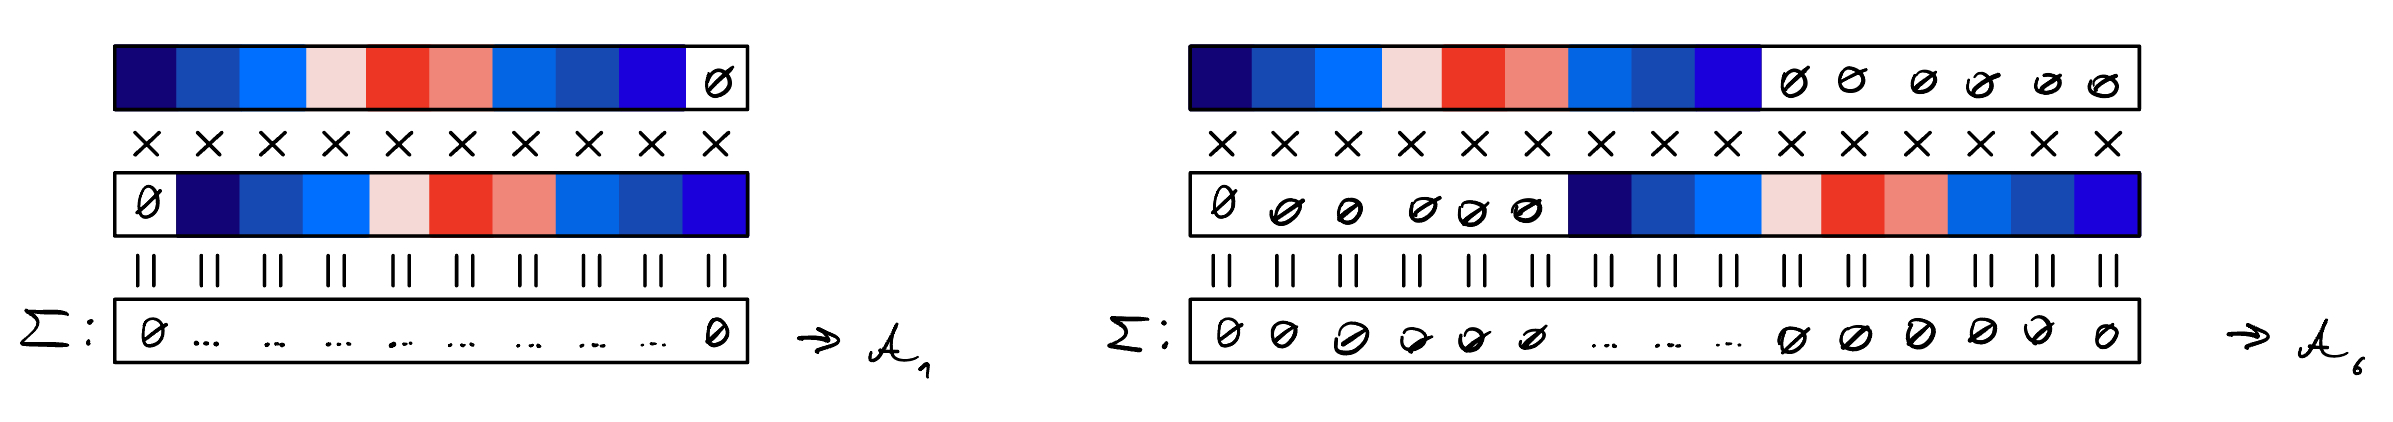
\includegraphics[width=0.9\textwidth]{figures/chap2/ACF_bound.jpeg}
    \caption{[CHANGE PICTURE TO BETTER VERSION] Boundary effects when computing the autocorrelation function on the whole signal. Since the signal is finite, the contributions on the borders are zero.}
    \label{fig:ACF_bound}
\end{figure}
\begin{figure}[h!]
    \centering
    \includegraphics[width=0.5\textwidth]{figures/chap2/ACF_window.jpeg}
    \caption{[CHANGE PICTURE TO BETTER VERSION] Windowed autocorrelation scheme. No boundary effects}
    \label{fig:ACF_window}
\end{figure}
It is then worth to limit the signal in a central window of length $2W$ and computing the ACF on the windowed signal. Taking as input the latter as $Z_0,\dots,Z_{2W-1}$, the output will be a series of values $\mathcal{A}_0,\dots,\mathcal{A}_{W}$ living in the spatial domain\footnote{While the FFT domain is made of frequencies, the ACF domain is instead made of lag values, corresponding to the spatial shifts of the signal.} such that:
\begin{equation*}
    \mathcal{A}_k = \frac{1}{2} \left( \frac{\sum_{n} Z_n Z_{n+k}}{\sqrt{\sum_{n} Z_n^2 \sum_{n} Z_{n+k}^2}} + \frac{\sum_{n} Z_n Z_{n-k}}{\sqrt{\sum_{n} Z_n^2 \sum_{n} Z_{n-k}^2}} \right)\, .
\end{equation*}
This formula computes the windowed autocorrelation by shifting the signal both to the left and to the right and then taking the average.
Both terms are normalized in order to get $\mathcal{A}_0 = 1$. The computation of this function on some simple signals is shown in App.\ \ref{chap:app_ACF}. Note that the sums run from $n = 0$ to $n = W-1$ and thus the length of the signal must be greater than $4W$: data that does not respect this condition will not be analyzed. A scheme is presented in Fig.\ \ref{fig:ACF_window}.

\subsection{FFT and ACF analysis}
Now, what we shall do is computing the FFT and the ACF on the data, taking care of the fact that it is necessary to separate the inside region (the bubble) from the outside one. This is done by relying on the fit routine results, mainly the shoulder centers and their widths.
We will also compute the transforms on the no-bubble shots. An example of the inside region zero-mean analysis for a selected sequence is presented in Fig.\ \ref{fig:inside_00}.
\begin{figure}[h!]
    \centering
    \includegraphics[width=0.75\textwidth]{figures/chap2/inside_day_0_seq_0.png}
    \caption{Example of FFT and ACF calculated in a sequence. The values for each shot are shown in the left plots with colormaps, while the averages on all shots are on the right. Note that before computing the transforms the data was set to zero-mean by subtracting its average.}
    \label{fig:inside_00}
\end{figure}
% One can probably (with a good eye) already see in the colormap plot that two or three vertical bands extend over all shots and appear at the same frequencies. This ensures that the FFT averaging is rightful.

Let us briefly discuss the behaviours of the computed FFTs and ACFs, considering that it is similar for all sequences and the example presented is a good one (see Fig.\ \ref{fig:inside_avg}). The FFT shows a peak at a frequency in the order of $k_{\rm FFT} \sim 0.01$ \unit{\per\micro\meter} and of width in the order of $\Delta k_{\rm FFT} \sim 0.1$ \unit{\per\micro\meter}. The ACF instead has a first peak at $\Delta x_{\rm ACF} \sim 10-11$ \unit{\micro\meter}. By comparing these results, one should see a correspondence, namely $k \sim 1/\Delta x$. However, by taking the inverse of the ACF peak values, one gets $k_{\rm ACF} \sim 0.1$ \unit{\per\micro\meter}, a frequency hidden in the FFT plot due to the broad peak. The reason for the peak broadness is probability the data noise, which is difficult to analyze properly. We will thus proceed by relying on the ACF for the remaining analysis.

\begin{figure}[t!]
    \centering
    \includegraphics[width=0.75\textwidth]{figures/chap2/inside_fft_avg.png}
    \caption{FFT and ACF profiles (computed with zero-mean data) averaged over all sequences with the same radiation coupling $\Omega_R$.}
    \label{fig:inside_avg}
\end{figure}

From now on, all shots will be considered, independently from days and sequences. What we shall proceed to do is studying the ACF parameters as functions of the bubble properties, such as the experimental waiting time and the bubble size, and of the experimental external parameters: the coupling $\Omega_R$ and the detuning $\delta$. 
The routine is the following:
\begin{enumerate}
    \item Gather all shots with the same $\Omega_R$ and save their bubble parameters
    \item Sort the shots based on the bubble property we are interested in
    \item Group the shots in blocks of a fixed length
    \item Compute the ACF for each shot in a block and take the average
    \item Plot the ACF averages for each block and fit them
\end{enumerate}
In particular, the ACF profiles can be fitted with a damped cosine of the form
\begin{equation*}
    \mathcal{A}_{\rm fit}(x) = (1 - \Delta)\cos(\frac{x}{\ell_2})\exp[-\left(\frac{x}{\ell_1}\right)^\alpha] + \Delta\, ,
\end{equation*}
with $\alpha = 1.7$ fine-tuned in order to catch the profile in the best way possible.\footnote{One could set $\alpha$ as a fit parameter, but this would result in a worse estimation of the length $\ell_1$.} An example is presented in Fig.\ \ref{fig:fit_time_inside}, where the shots are grouped by time. The fit parameters retrieved from the fit are in Fig.\ \ref{fig:param_time_inside}.

\begin{figure}
    \centering
    \includegraphics[width = \textwidth]{figures/chap2/fit_time_inside.png}
    \caption{ACF average profiles of shots grouped by time in 10 blocks and fitted with the damped cosine for each value of $\Omega_R$.}
    \label{fig:fit_time_inside}
\end{figure}
\begin{figure}
    \centering
    \includegraphics[width = \textwidth]{figures/chap2/param_time_inside.png}
    \caption{Fit parameters $\ell_1$, $\Delta$ (off) and $\ell_2$ of shots grouped by time.}
    \label{fig:param_time_inside}
\end{figure}

% \subsection{Border alignment}
